\section{Continuous Integration/Delivery}
\subsection{GitHub Actions}

allg. actions warum kosten
\subsubsection{Build IOS}
\author{Martin Hausleitner}

\subsubsection{Build Android}

\subsection{Fastline}
\subsubsection{Build Number increment}
\subsection{Firebase App Distribution}

\section{Mobile Anwendung}
\subsection{Dateistruktur}
\author{Martin Hausleitner}
In Flutter gibt es keine fixe Dateistruktur für eine App,
man kann seine Struktur also selbst überlegen und gestalten.
Im Folgenden beschreibe ich, wie wir unsere Dateistruktur
für eine Flutter-App aufgebaut haben.

In Flutter gibt es keine feste Dateistruktur, stattdessen kann man die Struktur der Dateien und Ordner selbst bestimmen. Für unser Flutter-Projekt haben wir uns für eine Struktur entschieden, die sich an bewährten Praktiken orientiert.

Unsere Dateistruktur sieht wie folgt aus:

\begin{itemize}
    \item \textbf{logic} - Hier befindet sich die Geschäftslogik der App, einschließlich der Firestore-Cloud-Funktionen und Repositories, die API-Aufrufe ausführen.
    \item \textbf{pages} - Hier werden Widgets entworfen, die jeweils eine Seite der App darstellen.
    \item \textbf{routes} - Hier werden die Routen definiert, die tiefere Links ermöglichen.
    \item \textbf{shared} - Hier werden UI-Widgets wie Buttons oder andere Widgets gespeichert, die oft wiederverwendet werden.
    \item \textbf{views} - Hier befinden sich Ansichten, die von mehreren Seiten der App verwendet werden können.
\end{itemize}

Im Nachhinein hätten wir die Dateistruktur anders gestaltet,
z.B. hätten wir das UI als eigenes Package definiert und die
pages und views besser unterteilt.

\subsection{State Management}
In Flutter gibt es verschiedene Möglichkeiten\cite{flutter-docs-interactive}\cite{flutter-state-management-blog}, um mit dem State Management umzugehen. State Management bezieht sich auf die Art und Weise, wie Daten innerhalb einer App verwaltet werden. In jeder App gibt es bestimmte Daten, die von verschiedenen Komponenten und Widgets verwendet werden und sich im Laufe der Zeit ändern können. State Management bezieht sich auf die Methoden, die verwendet werden, um diese Daten innerhalb der App zu verwalten und zu aktualisieren.
\author{Martin Hausleitner}

\subsubsection{GetX}
\author{Martin Hausleitner}

GetX verwendet ein reaktives Ansatz zur Verwaltung des Zustands, was bedeutet, dass Änderungen im Zustand automatisch die UI aktualisieren, ohne dass der Entwickler manuell Code schreiben muss, um diese Aktualisierungen durchzuführen. Dies spart viel Entwicklungszeit und macht es einfach, auf Benutzerinteraktionen zu reagieren.

Mit GetX können wir auch eine einheitliche Datenquelle haben, auf die alle Komponenten zugreifen können, was die Wartung und Erweiterung der Anwendung erleichtert. Darüber hinaus bietet GetX auch eine einfache Möglichkeit, Abhängigkeiten zu verwalten und Zustandsinformationen zwischen Bildschirmen zu teilen.

Insgesamt hat uns die Verwendung von GetX im Flutter-Framework sehr geholfen, eine effektive und skalierbare Anwendung zu erstellen, die auf die Bedürfnisse unserer Benutzer abgestimmt ist.
\author{Sandin Habibovic}
getx controller service etc...


\subsection{Authentifizierung}
\author{Sandin Habibovic}

\subsubsection{Anmelde Flow}
\author{Sandin Habibovic}

Diagram
erklärung
screenshots
\subsubsection{Regestrierungs Flow}
\author{Sandin Habibovic}


Diagram
erklärung
screenshots


\subsubsection{Firebase Authentifizierung}
\author{Sandin Habibovic}

allg.


\subsection{Feed}
\author{Sandin Habibovic}
foto
aufbau

\subsection{Beiträge}
\author{Sandin Habibovic}
Beiträge sind das Hauptkommunikationsmittel auf der App. Jedem Beitrag muss ein Titel, eine Beschreibung und eine Reichweite, unter der, der Beitrag sichtbar ist, angegeben werden. Weiters ist es möglich einem Beitrag ein Bild und Tags anzuhängen.

\subsubsection{Kategorien}
\author{Sandin Habibovic}
Um Beiträge besser zuordnen zu können, muss der User den Beitrag vor dem Veröffentlichen in eine bestimmte Kategorie einteilen. Diese Kategorien ermöglichen es Usern, die Art Ihrer Anfrage ihm vorhinein besser zu spezifizieren und die Suche nach Beiträgen einer bestimmten Art zu vereinfachen. Bestimmte Kategorien werden weiters in Unterkategorien aufgeteilt, da diese ein zu weit gefächertes Genre an Anfragen umfassen.

Es existieren folgende Kategorien bzw. Unterkategorien:

\begin{compactitem}
    \item Mitteilung
    \begin{compactitem}
        \item Frage
        \item Appell
        \item Warnung
        \item Empfehlung
        \item Gefunden
    \end{compactitem}
    \item Suche
    \begin{compactitem}
        \item Hilfe
        \item Verloren
    \end{compactitem}
    \item Ausleihen
    \item Event
\end{compactitem}



Mitteilung:
Die Kategorie der Mitteilung dient dazu die Nachbarn über ein bestimmtes Ereignis oder Meldung zu informieren oder zu befragen.

Suche:
Die Kategorie der Suche dient dazu mit den Nachbarn im Falle einer Hilfesuche oder eines verloren gegangenen Objekts in Kontakt zu treten.

Ausleihen:
Die Kategorie des Ausleihens dient dazu die Nachbarn nach der Erlaubnis, sich ein bestimmtes Werkzeug oder Objekt ausborgen zu dürfen, zu bitten.

Event:
Die Kategorie des Events dient dazu die Nachbarn auf eine bestimmte Veranstaltung aufmerksam zu machen.


\subsubsection{Tags}
\author{Sandin Habibovic}
Als Tag wird ein Schlüsselwort beschrieben, was man an ein Informationsgut anhängen kann, um es besser beschreiben zu können und/oder besser auffindbar zu machen. In der App werden Tags als eine Erweiterung der Kategorien verwendet, um es Usern zu ermöglichen Ihren Beitrag einem selbstdefinierten Typ zuzuordnen.

\subsubsection{Info}
\author{Sandin Habibovic}
Jeder Beitrag hat eine eigene Sektion, wo wichtige Entscheidungsinformationen angegeben werden, wie der Stadtteil und die ungefähre Entfernung zum gegebenen Nachbarn und das Erstelldatum des Beitrags.

\subsubsection{Kommentare}
\author{Sandin Habibovic}
Die Kommentarfunktion ermöglicht es den Usern unter einem Beitrag Ihre Meinung, Feedback oder sonstiges zu hinterlassen.

\subsubsection{Beitrag oder Kommentar Melden}
\author{Sandin Habibovic}
Um auf unangebrachte Beiträge oder Kommentare schnell reagieren zu können, gibt es die Möglichkeit Beiträge oder Kommentare zu melden. Diese Meldungen werden auf Firestore gespeichert und können dann im Einzelnen überprüft werden. Fürs Melden muss ein Grund ausgewählt und eine genauere Beschreibung angegeben werden.
Gründe fürs Melden eines Beitrags oder Kommentars:

\begin{compactitem}
    \item Unangebrachter Inhalt
    \item Belästigung
    \item Betrug
    \item Spam
    \item Sonstiges
\end{compactitem}

\subsection{Filter}
\author{Sandin Habibovic}
Filtern nach Kategorien
Ordnen nach Likes oder Datum
Absteigend oder aufsteigend sortieren

\subsection{Suche}
\subsection{Typesense}
\subsection{Algolia}
diagram
\subsubsection{Firestore Sync}

\subsubsection{Algolia SDK}


\subsection{Chat}
package genommen warum
\subsubsection{Flyer Package}

\subsection{Profil}
\author{Sandin Habibovic}
Was wird angezeigt?
Name, User Public Info, Posts von User

\subsubsection{Profil Melden}
\author{Sandin Habibovic}

\subsection{Benachrichtigungen}
\author{Sandin Habibovic}
Grund und Funktionsweise von Benachrichtigungen
diagram beschreibung
\subsection{Einstellungen}
\author{Sandin Habibovic}
Email/Passwort ändern, Konto löschen, Sprache einstellen, Benachrichtigungen ein/ausschalten
\subsection{Feedback}
\author{Martin Hausleitner}
feedback feature beschreiben


\section{UI/UX Design}
Das UI/UX-Design einer App ist von entscheidender Bedeutung für den Erfolg der App und die Zufriedenheit der Benutzer. Insbesondere bei einer Social-Media-Nachbarschafts-App ist ein gut durchdachtes UI/UX-Design unerlässlich, um eine positive Benutzererfahrung zu gewährleisten.

Ein gutes UI-Design ist wichtig, um sicherzustellen, dass die Benutzer die App einfach und intuitiv bedienen können. Es sollte eine klare Struktur und Navigation haben, damit die Benutzer schnell zu den gewünschten Funktionen gelangen können. Wenn die Benutzer die App als kompliziert oder verwirrend empfinden, werden sie möglicherweise frustriert und geben die Nutzung der App auf.

Auch ein gutes UX-Design ist wichtig, um sicherzustellen, dass die Benutzer mit der App zufrieden sind. Es sollte eine ansprechende und ansprechende Benutzeroberfläche bieten, die dem Benutzer ein angenehmes Nutzungserlebnis vermittelt. Wenn die Benutzer die App als langweilig oder uninteressant empfinden, werden sie möglicherweise nicht wiederkommen.

Darüber hinaus sollte das UI/UX-Design einer Social-Media-Nachbarschafts-App bestimmte Funktionen und Merkmale berücksichtigen, die für eine erfolgreiche Community-Plattform erforderlich sind. Beispielsweise sollte es einfach sein, Beiträge zu erstellen und zu teilen, auf Kommentare zu antworten und Nachrichten an andere Benutzer zu senden. Es sollte auch Möglichkeiten geben, um Benutzerprofile zu erstellen und zu verwalten sowie umfassende Datenschutz- und Sicherheitsfunktionen zu bieten.

Insgesamt ist das UI/UX-Design einer Social-Media-Nachbarschafts-App von entscheidender Bedeutung für den Erfolg der App und die Zufriedenheit der Benutzer. Es ist wichtig, dass das Design auf die Bedürfnisse und Anforderungen der Benutzer zugeschnitten ist und ein einfaches, intuitives und ansprechendes Nutzungserlebnis bietet.
\author{Martin Hausleitner}
\subsection{Inspiration}
Während des Designprozesses für die App habe ich Recherchen im Bereich App-Design durchgeführt. Mein Ziel war es, die App so intuitiv wie möglich zu gestalten, um eine benutzerfreundliche Erfahrung zu gewährleisten. Dazu habe ich mich an bekannten Social-Media-Apps orientiert, wie zum Beispiel Twitter, Instagram und TikTok, die bereits auf dem Markt sehr erfolgreich sind und von vielen Menschen vertraut genutzt werden.

Darüber hinaus hat auch die erfolgreichste Nachbarschafts-App in Deutschland, "Nebenan", viel zur Grundlage der App beigetragen. Allerdings habe ich festgestellt, dass ihre App sehr kompliziert aufgebaut und unübersichtlich ist, was für uns eine Chance darstellte, es besser zu machen.

Zusätzlich haben wir uns von Websites wie Dribble und Mobbin inspirieren lassen, die uns geholfen haben, ein einfaches und schlichtes Design für die App zu entwickeln. Insgesamt war die Recherche und Inspiration für das Design der App ein wichtiger Schritt, um sicherzustellen, dass unsere Benutzer eine ansprechende und intuitive Erfahrung haben.

\subsection{Prototyping}
Prototyping ist ein wichtiger Schritt bei der Entwicklung von mobilen Apps. Es ermöglicht Entwicklern, Designern und anderen Stakeholdern, eine frühzeitige Vorstellung davon zu bekommen, wie die App funktionieren wird und wie sie aussehen wird. Durch die Erstellung eines Prototyps können auch Fehler im Design und in der Funktionalität identifiziert werden, bevor die App in die eigentliche Entwicklung geht.

Es gibt verschiedene Arten von Prototypen, darunter Low-Fidelity- und High-Fidelity-Prototypen. Low-Fidelity-Prototypen sind einfache Skizzen oder Wireframes, die nur die grundlegenden Funktionen und das Layout der App abbilden. High-Fidelity-Prototypen sind detaillierter und können interaktive Funktionen und Designelemente enthalten.

Es gibt viele Tools und Plattformen, die zur Erstellung von Prototypen verwendet werden können. Ein Beispiel ist Adobe XD, das es Entwicklern und Designern ermöglicht, schnelle und einfache Prototypen zu erstellen. Andere Tools wie Sketch, Figma oder InVision sind ebenfalls beliebt.

Der Vorteil von Prototyping ist, dass es Entwicklern und Designern ermöglicht, frühzeitig Feedback von Benutzern zu erhalten und Änderungen vorzunehmen, bevor die App tatsächlich entwickelt wird. Außerdem können Entwickler und Designer Zeit und Ressourcen sparen, indem sie sich auf die richtigen Funktionen und das richtige Design konzentrieren und unnötige Funktionen und Designs vermeiden.

Im Fall von Flutter als Entwicklungsplattform für die App ist das Prototyping ebenfalls wichtig. Flutter bietet verschiedene Widgets und Design-Tools, mit denen Entwickler schnell und einfach Designelemente erstellen und implementieren können. Durch ein gut durchdachtes Prototyping kann Zeit und Aufwand beim Entwickeln gespart werden, da Design-Entscheidungen bereits getroffen wurden und Entwickler sich auf die Umsetzung konzentrieren können.

Insgesamt ist Prototyping ein unverzichtbarer Schritt bei der Entwicklung von mobilen Apps. Es ermöglicht Entwicklern und Designern, frühzeitig Feedback von Benutzern zu erhalten und Änderungen vorzunehmen, bevor die App tatsächlich entwickelt wird. Durch die Verwendung von Tools wie Adobe XD, Sketch oder Figma können Prototypen schnell und einfach erstellt werden, was Zeit und Ressourcen spart. Prototyping ist auch für die Verwendung von Flutter als Entwicklungsplattform wichtig, da es Entwicklern ermöglicht, Zeit und Aufwand zu sparen und sich auf die Umsetzung zu konzentrieren.
\subsubsection{Framer}
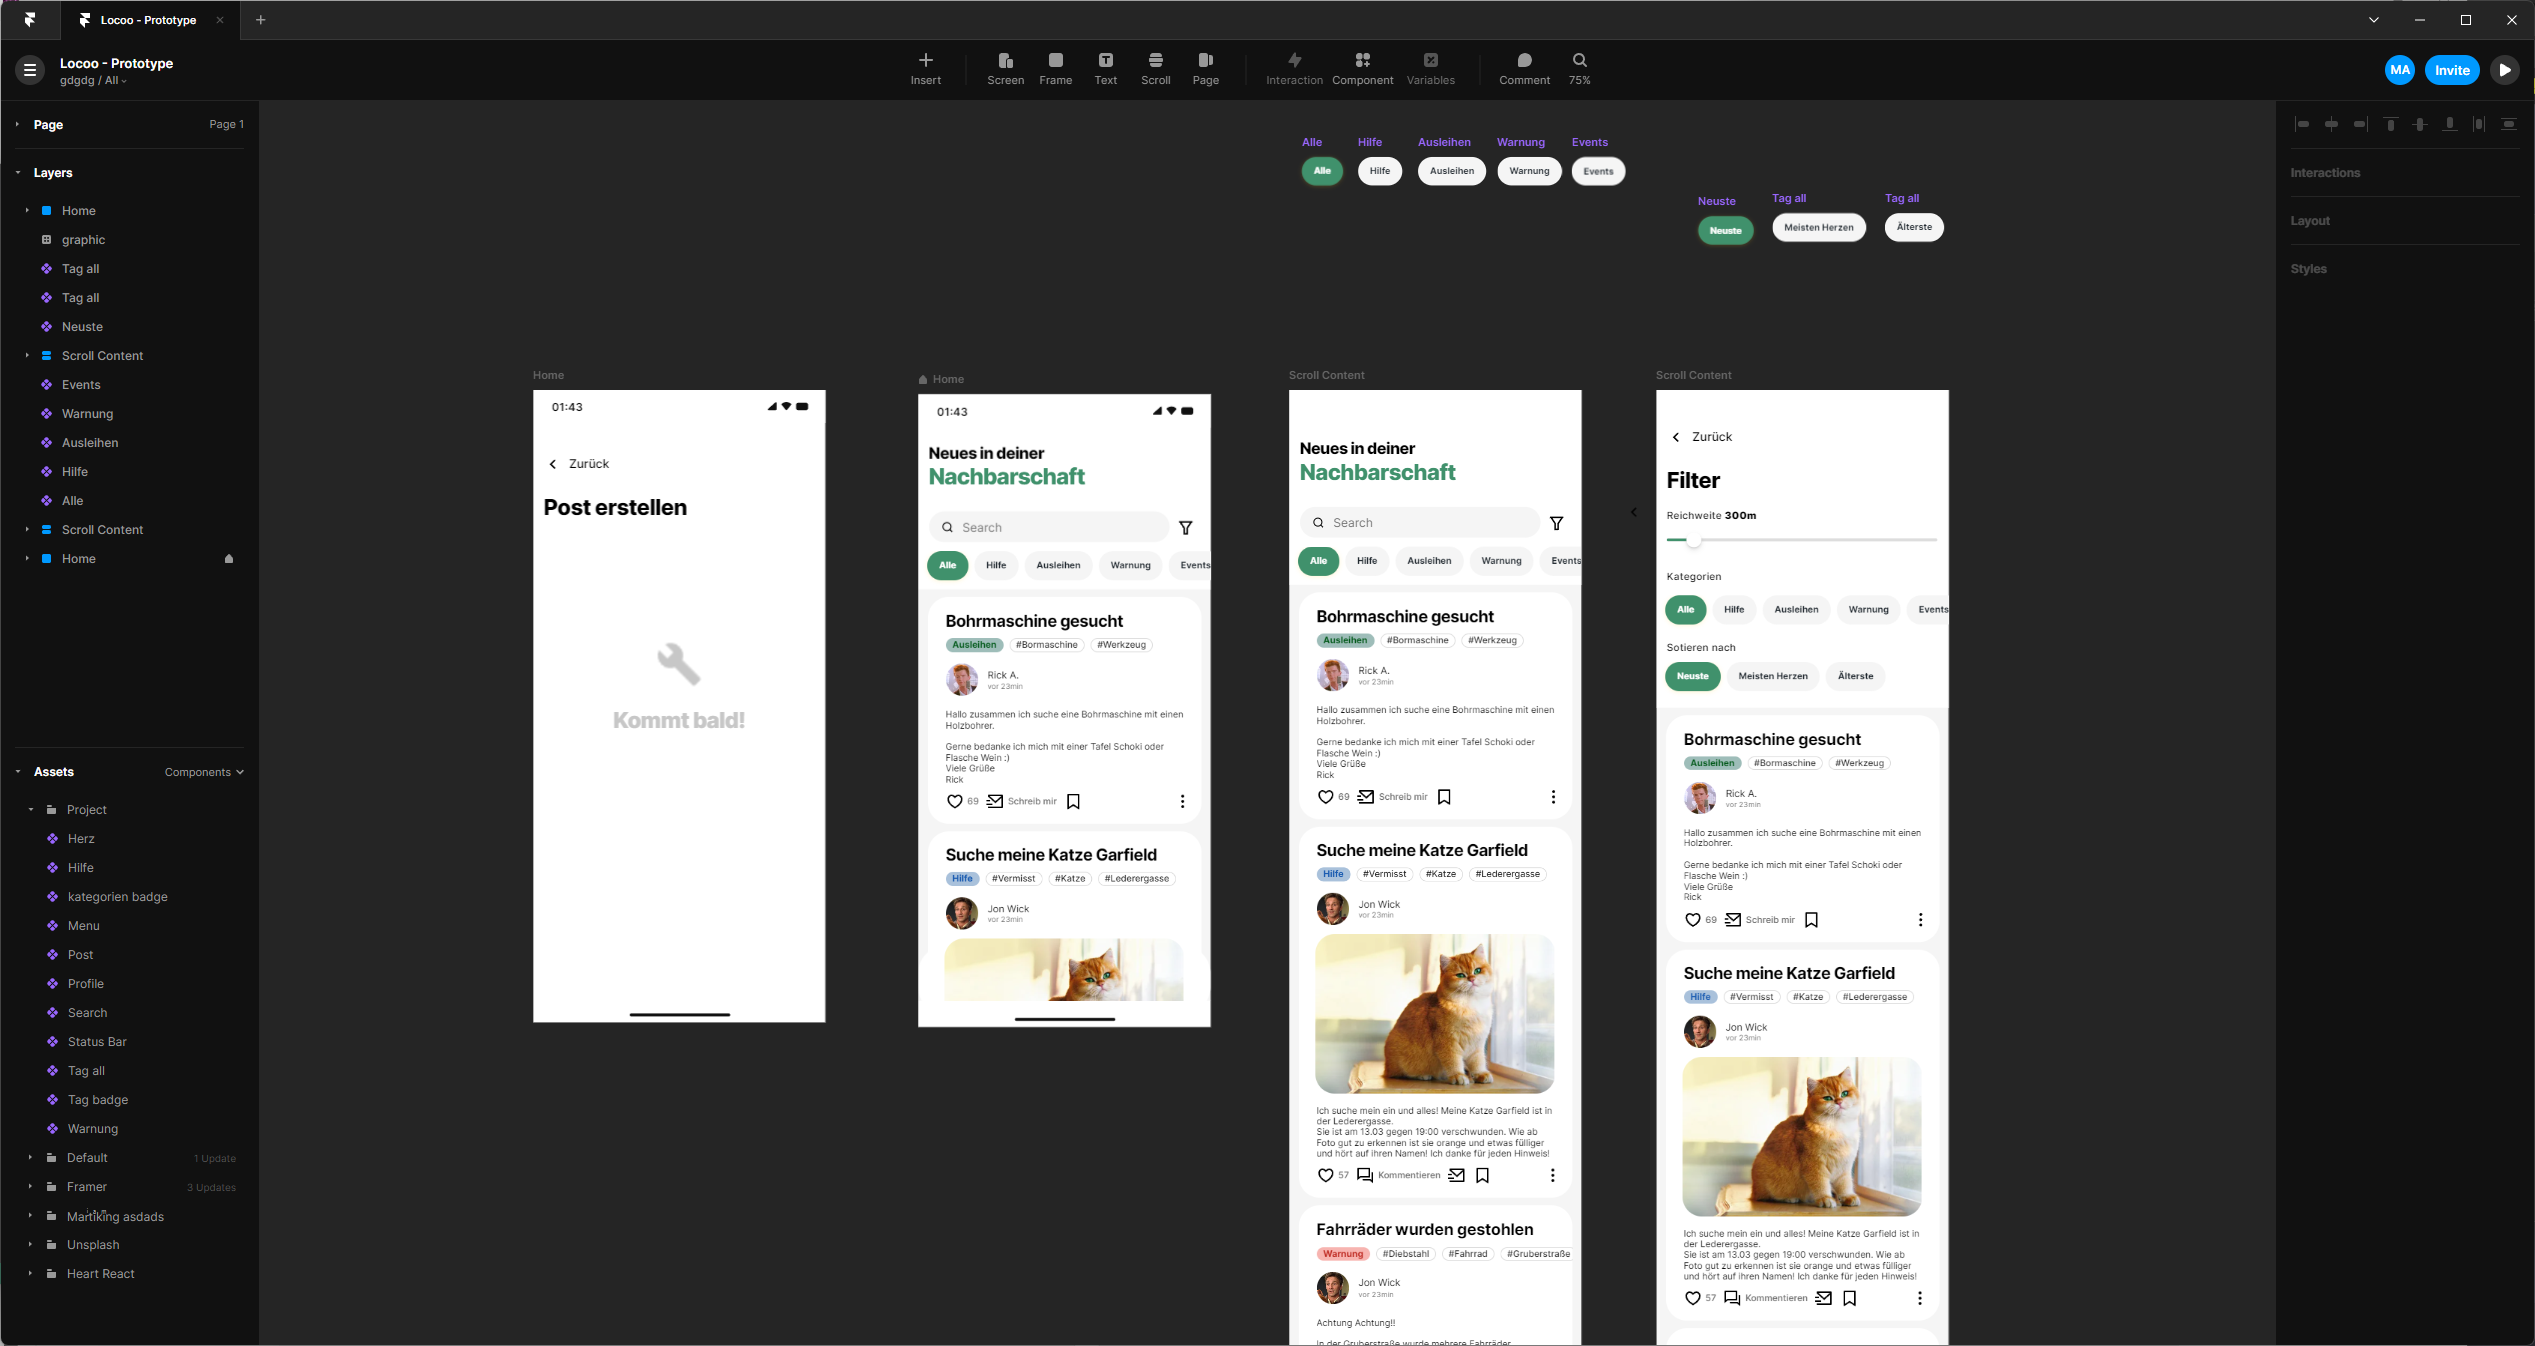
\includegraphics[width=0.95\textwidth]{pics/nochba-framer-prototype-screenshot.png}


Framer ist eine Software, die es Benutzern ermöglicht, schnell und einfach ansprechende Prototypen von mobilen Anwendungen und Websites zu erstellen. Das Tool wurde ursprünglich als Prototyping-Tool für Designer entwickelt, um Designs schnell zu testen und zu verfeinern, bevor sie in die Entwicklung übergehen.

Erfolgreiche Apps wie Spotify haben Framer im Rahmen ihres
Prototyping-Prozesses verwendet, um schnell und effizient
funktionierende App-Designs zu erstellen. Framer ist eine
schnelle und effiziente Möglichkeit, um Ideen in die Tat
umzusetzen, ohne sich durch langwierige Entwicklungsprozesse
zu quälen.

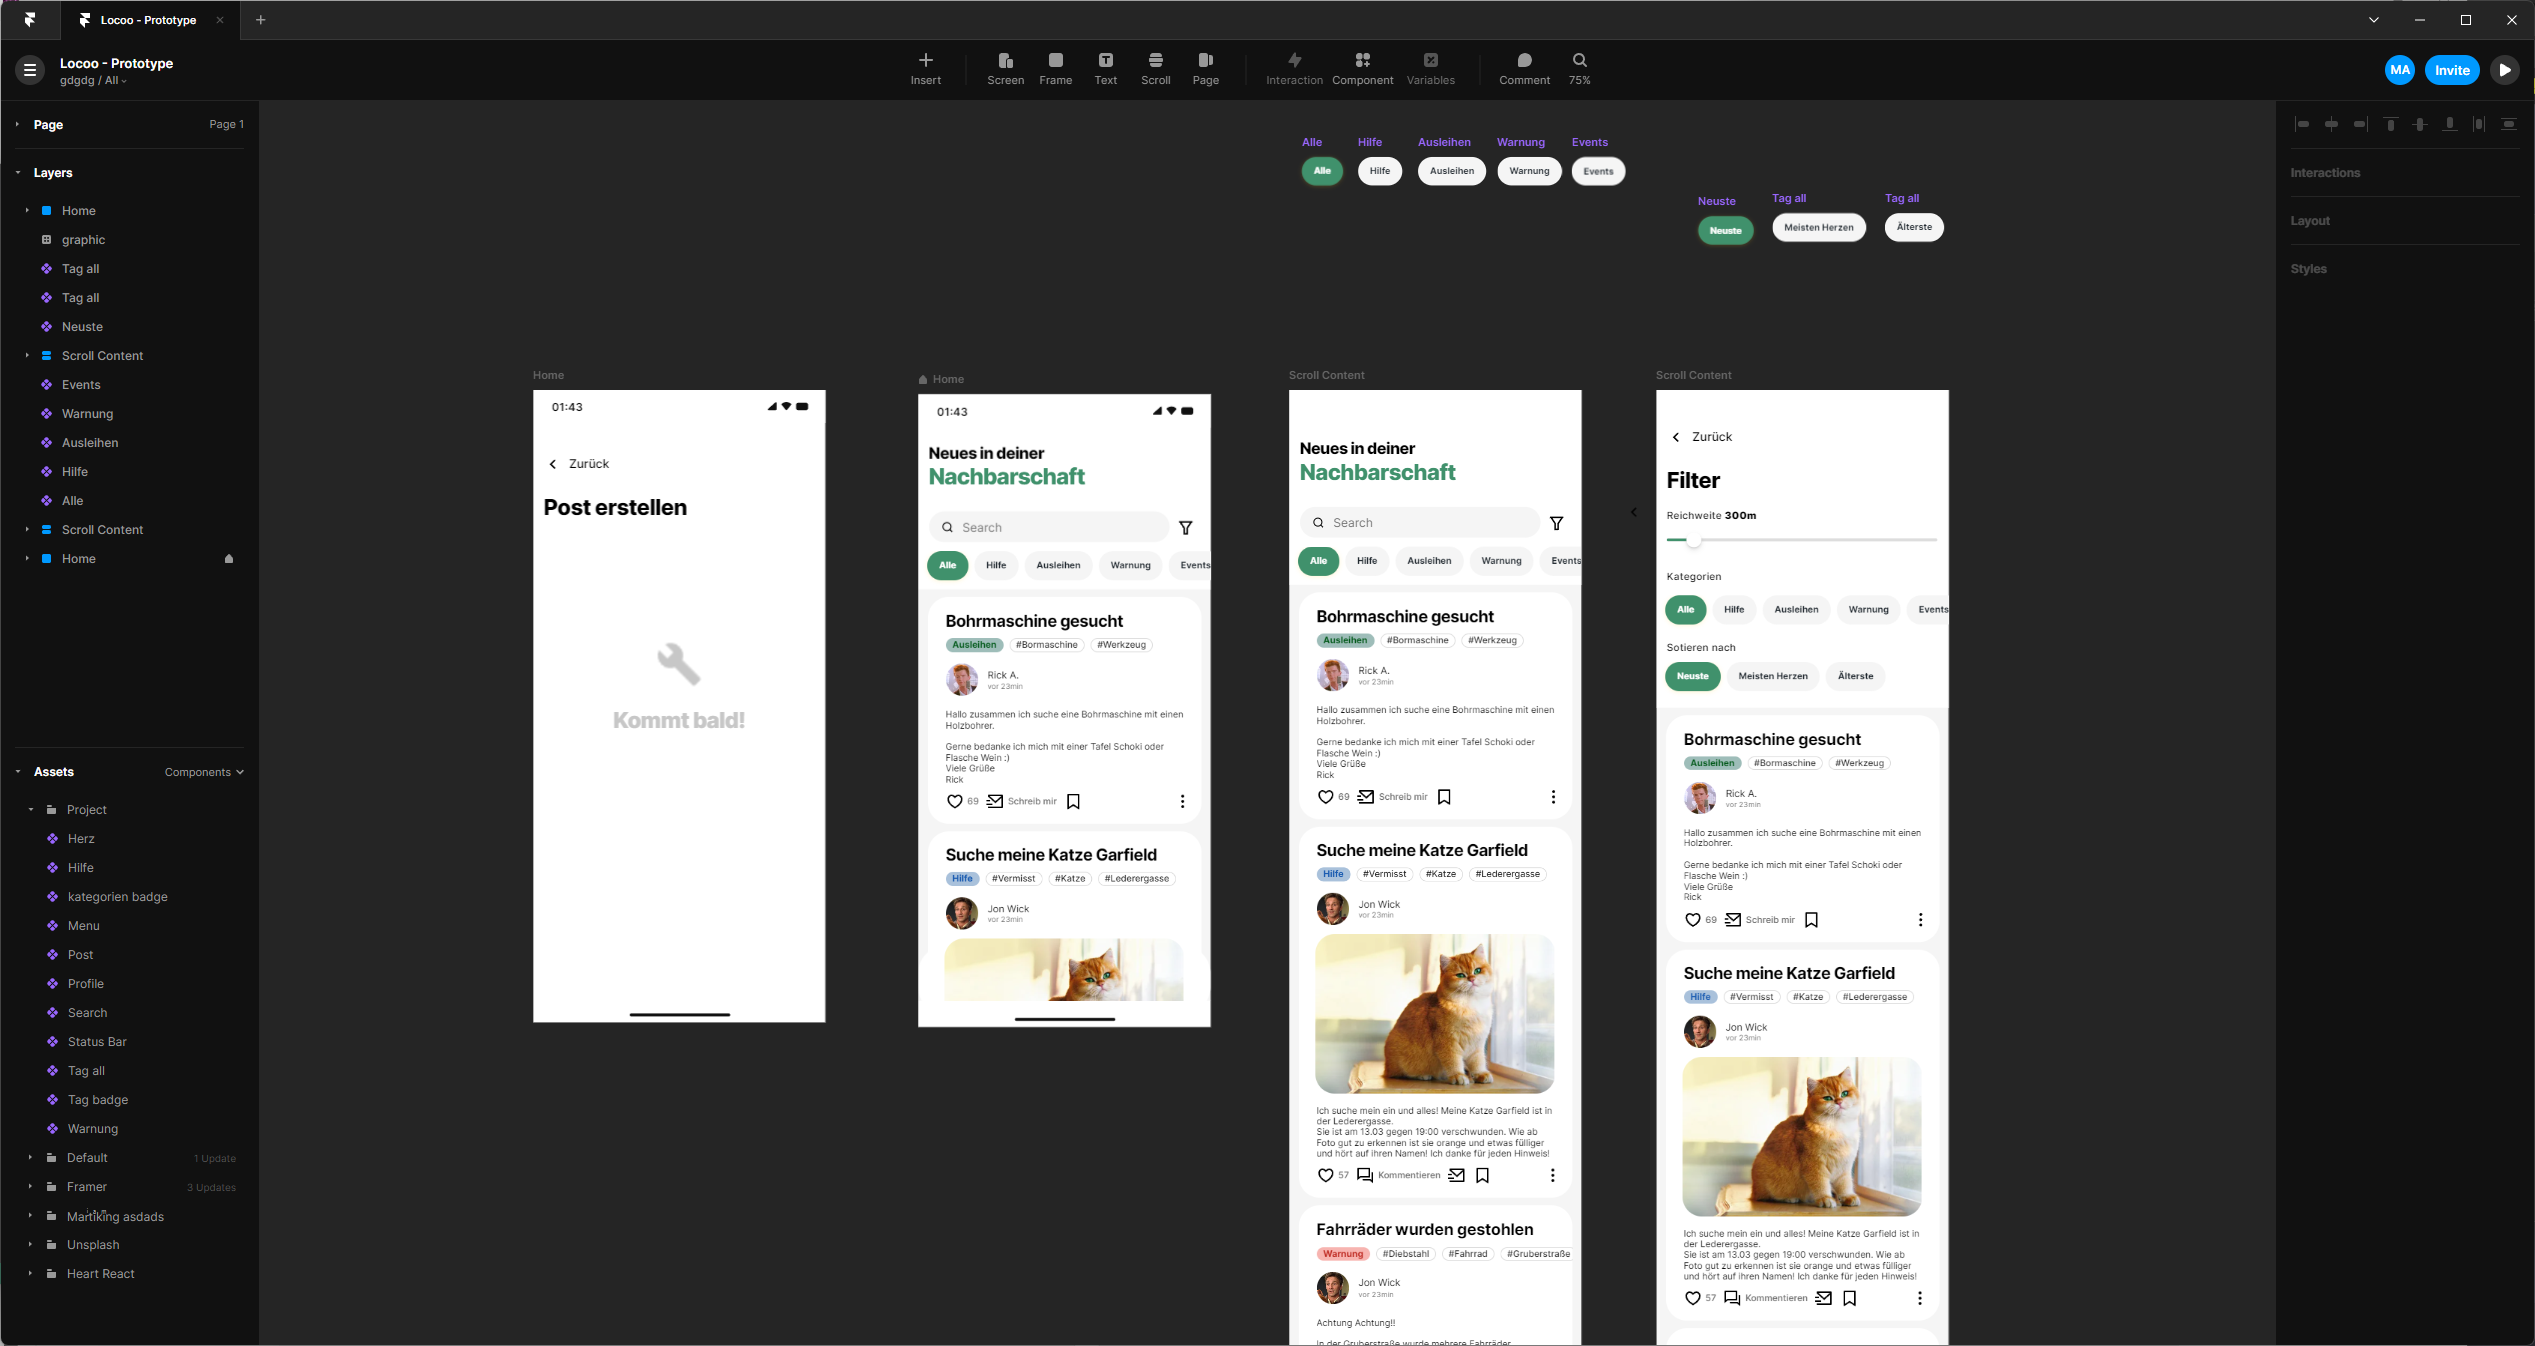
\includegraphics[width=0.95\textwidth]{pics/nochba-framer-prototype-screenshot.png}


Framer wurde während des Hackerthon Linz hackt verwendet, um den ersten Prototypen zu erstellen. Die Wahl von Framer war aufgrund seiner Geschwindigkeit und Effizienz in der Erstellung von funktionsfähigen App-Designs und der Erfahrung, die der Benutzer bereits mit dem Tool hatte, getroffen worden.

Seit der Erstellung des ersten Prototyps hat sich das Geschäftsmodell von Framer jedoch geändert. Es ist jetzt ein Website-Baukasten, der es Benutzern ermöglicht, einfach und schnell ansprechende Websites zu erstellen, ohne Kenntnisse in der Webentwicklung zu benötigen. Obwohl es nun als Website-Baukasten fungiert, behält Framer immer noch einige seiner Kernfunktionen als Prototyping-Tool bei, was es zu einer guten Option für Designer und Entwickler macht, die schnell Prototypen erstellen möchten.

Insgesamt hat Framer gezeigt, dass es ein schnelles und effektives Tool ist, um Designideen in die Tat umzusetzen. Obwohl es nun als Website-Baukasten fungiert, ist es immer noch eine nützliche Option für Designer und Entwickler, die schnell und einfach Prototypen erstellen möchten.

\subsubsection{Adobe XD}
Als ich zum ersten Mal mit Framer arbeitete, war ich begeistert von den vielen Features und Möglichkeiten, die es bietet. Aber im Laufe der Zeit stellte ich fest, dass es für mein Projekt zu aufwändig war und ich nach einer einfacheren Lösung suchte. So bin ich auf Adobe XD umgestiegen, ein Tool, mit dem ich schon jahrelange Erfahrung hatte.

Obwohl Adobe XD nicht so viele Features wie Framer bietet,
ist es aufgrund seiner Einfachheit und
Benutzerfreundlichkeit ein ideales Tool, um schnell einen
Prototypen zu erstellen. Ich hatte alle Hauptscreens
fertig gestaltet, bevor wir mit der Entwicklung mit Flutter
begannen. Die anderen wichtigen Screens habe ich dann
später gestaltet, als ich mit Flutter vertrauter war und
besser abschätzen konnte, wie aufwändig es in Flutter
umzusetzen war.

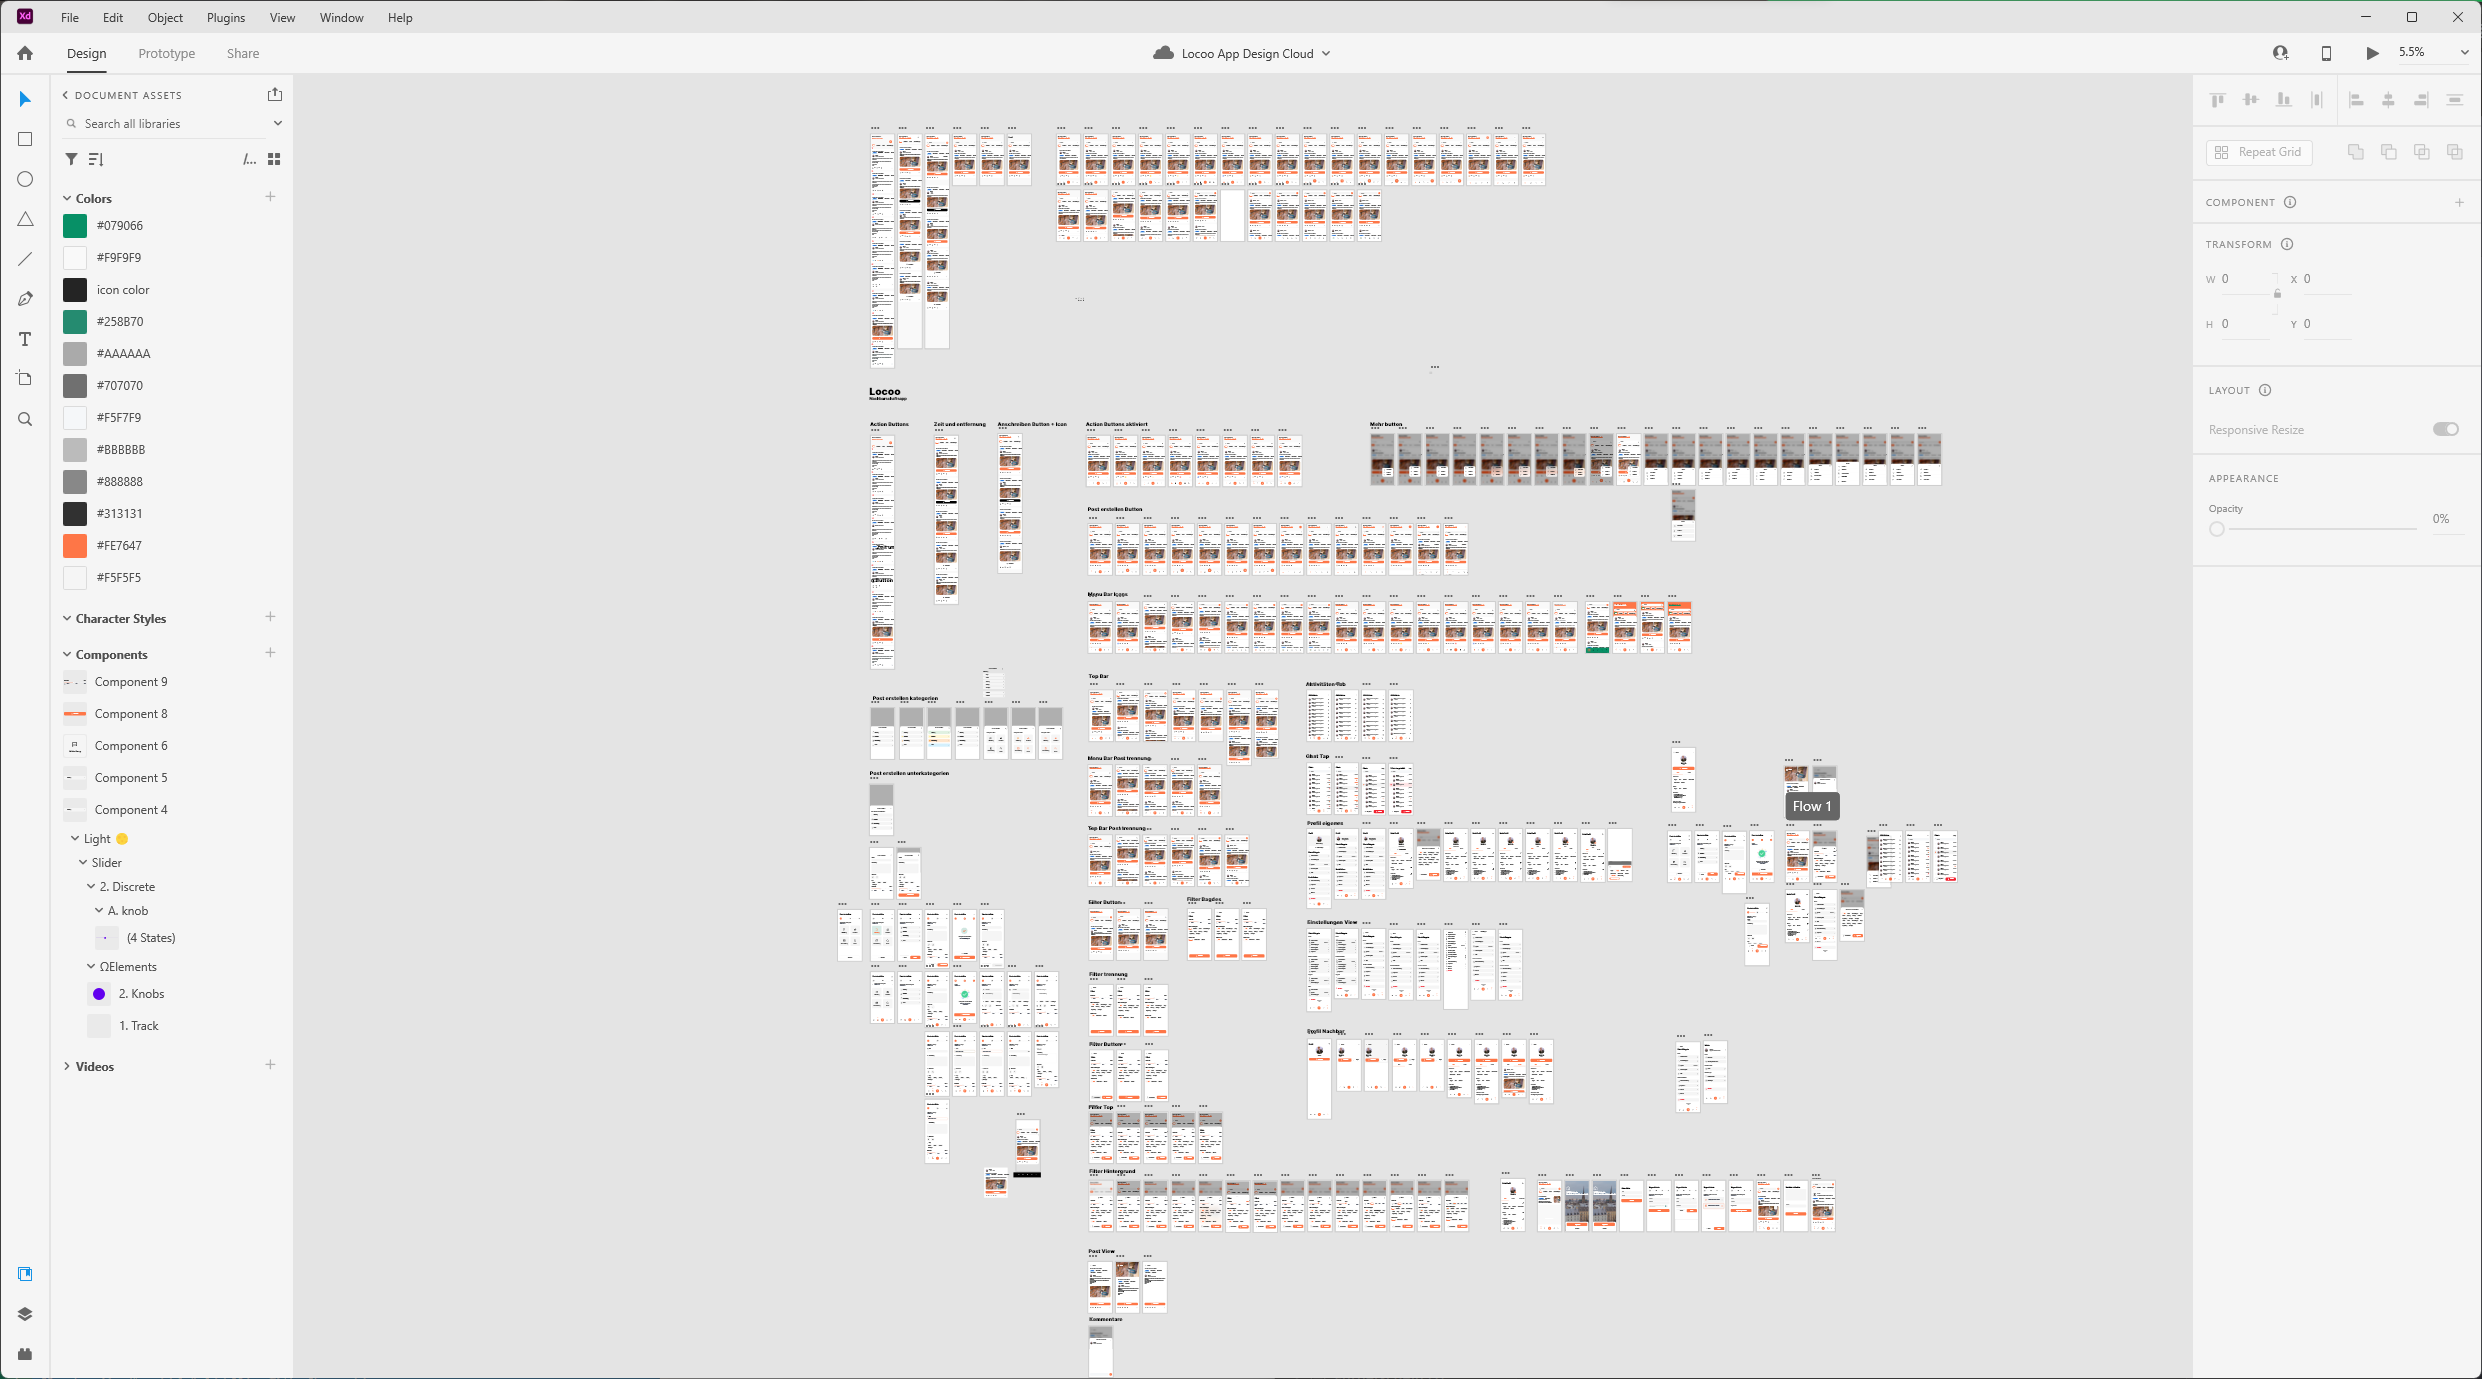
\includegraphics[width=0.95\textwidth]{pics/nochba-adobe-xd-protoype-screenshot.png}


Wie man auf dem obigen Bild sehen kann, ist unser Prototyp
eine Sammlung verschiedener Designs und Evolutionen des
Designs. Adobe XD war für unser Projekt perfekt, da ich der
alleinige Designer war und somit keine
Kollaborationsfunktion benötigte. Allerdings, da ich jetzt
mit dem bekanntesten Designtool Figma vertraut bin und es billiger ist, wenn mehrere
Personen an einem Design arbeiten und auch mehr Funktionen
bietet, würde ich aktuell mit Figma weiterarbeiten.

Zusammenfassend lässt sich sagen, dass Adobe XD ein mächtiges Tool für UI/UX-Designer ist, das einfach zu bedienen und ideal für kleine bis mittelgroße Projekte ist. Es bietet zwar nicht so viele Funktionen wie andere Tools, ist aber für schnelle Prototypenerstellung und einfache Zusammenarbeit mit Entwicklern und Stakeholdern sehr gut geeignet.

\subsection{Design}
allg.


\subsubsection{Farben}
farben history
warum orange
\subsubsection{Icons}
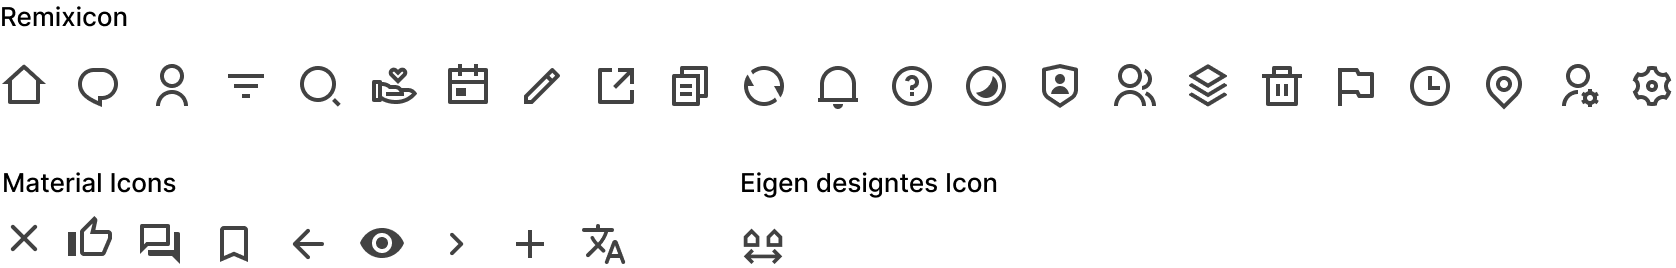
\includegraphics[width=1\textwidth]{pics/icons.png}
In der Abbildung oben sind alle verwendeten Icons in unserer App zu sehen. Es war uns ein wichtiges Anliegen, die App mit so vielen Icons wie möglich auszustatten, um die Bedienung intuitiver und benutzerfreundlicher zu gestalten. Nachdem wir uns mehrere Icon-Packs angesehen hatten, haben wir uns hauptsächlich für die frei verfügbaren Remixicons entschieden. Uns war wichtig, ein eher unbekanntes Icon-Pack zu verwenden, um unsere App von anderen abzuheben und ihr ein einzigartiges Aussehen zu geben. Besonders das verspielte, runde Design hat uns gut gefallen. Ein weiterer großer Vorteil von Remixicons ist, dass es ein Flutter-Paket gibt, was die Implementierung in Flutter vereinfacht hat.

Obwohl Remixicons über 2.271 Icons verfügt, haben uns bei einigen Icons die Material Icons von Google besser gefallen. Daher haben wir einige Icons von Google Material Icons verwendet, insbesondere die abgerundeten Icons, um das Design insgesamt nicht zu hart erscheinen zu lassen. Als ich kein passendes Icon finden konnte, um den Abstand zwischen zwei Nachbarn zu symbolisieren, habe ich mich selbst daran gesetzt, ein passendes Icon im Stil der anderen zu entwerfen.
\subsubsection{Fonts}
fotos von fonts
welche fonts
wie ist due typrographie aufgebaut
\subsubsection{Logo}

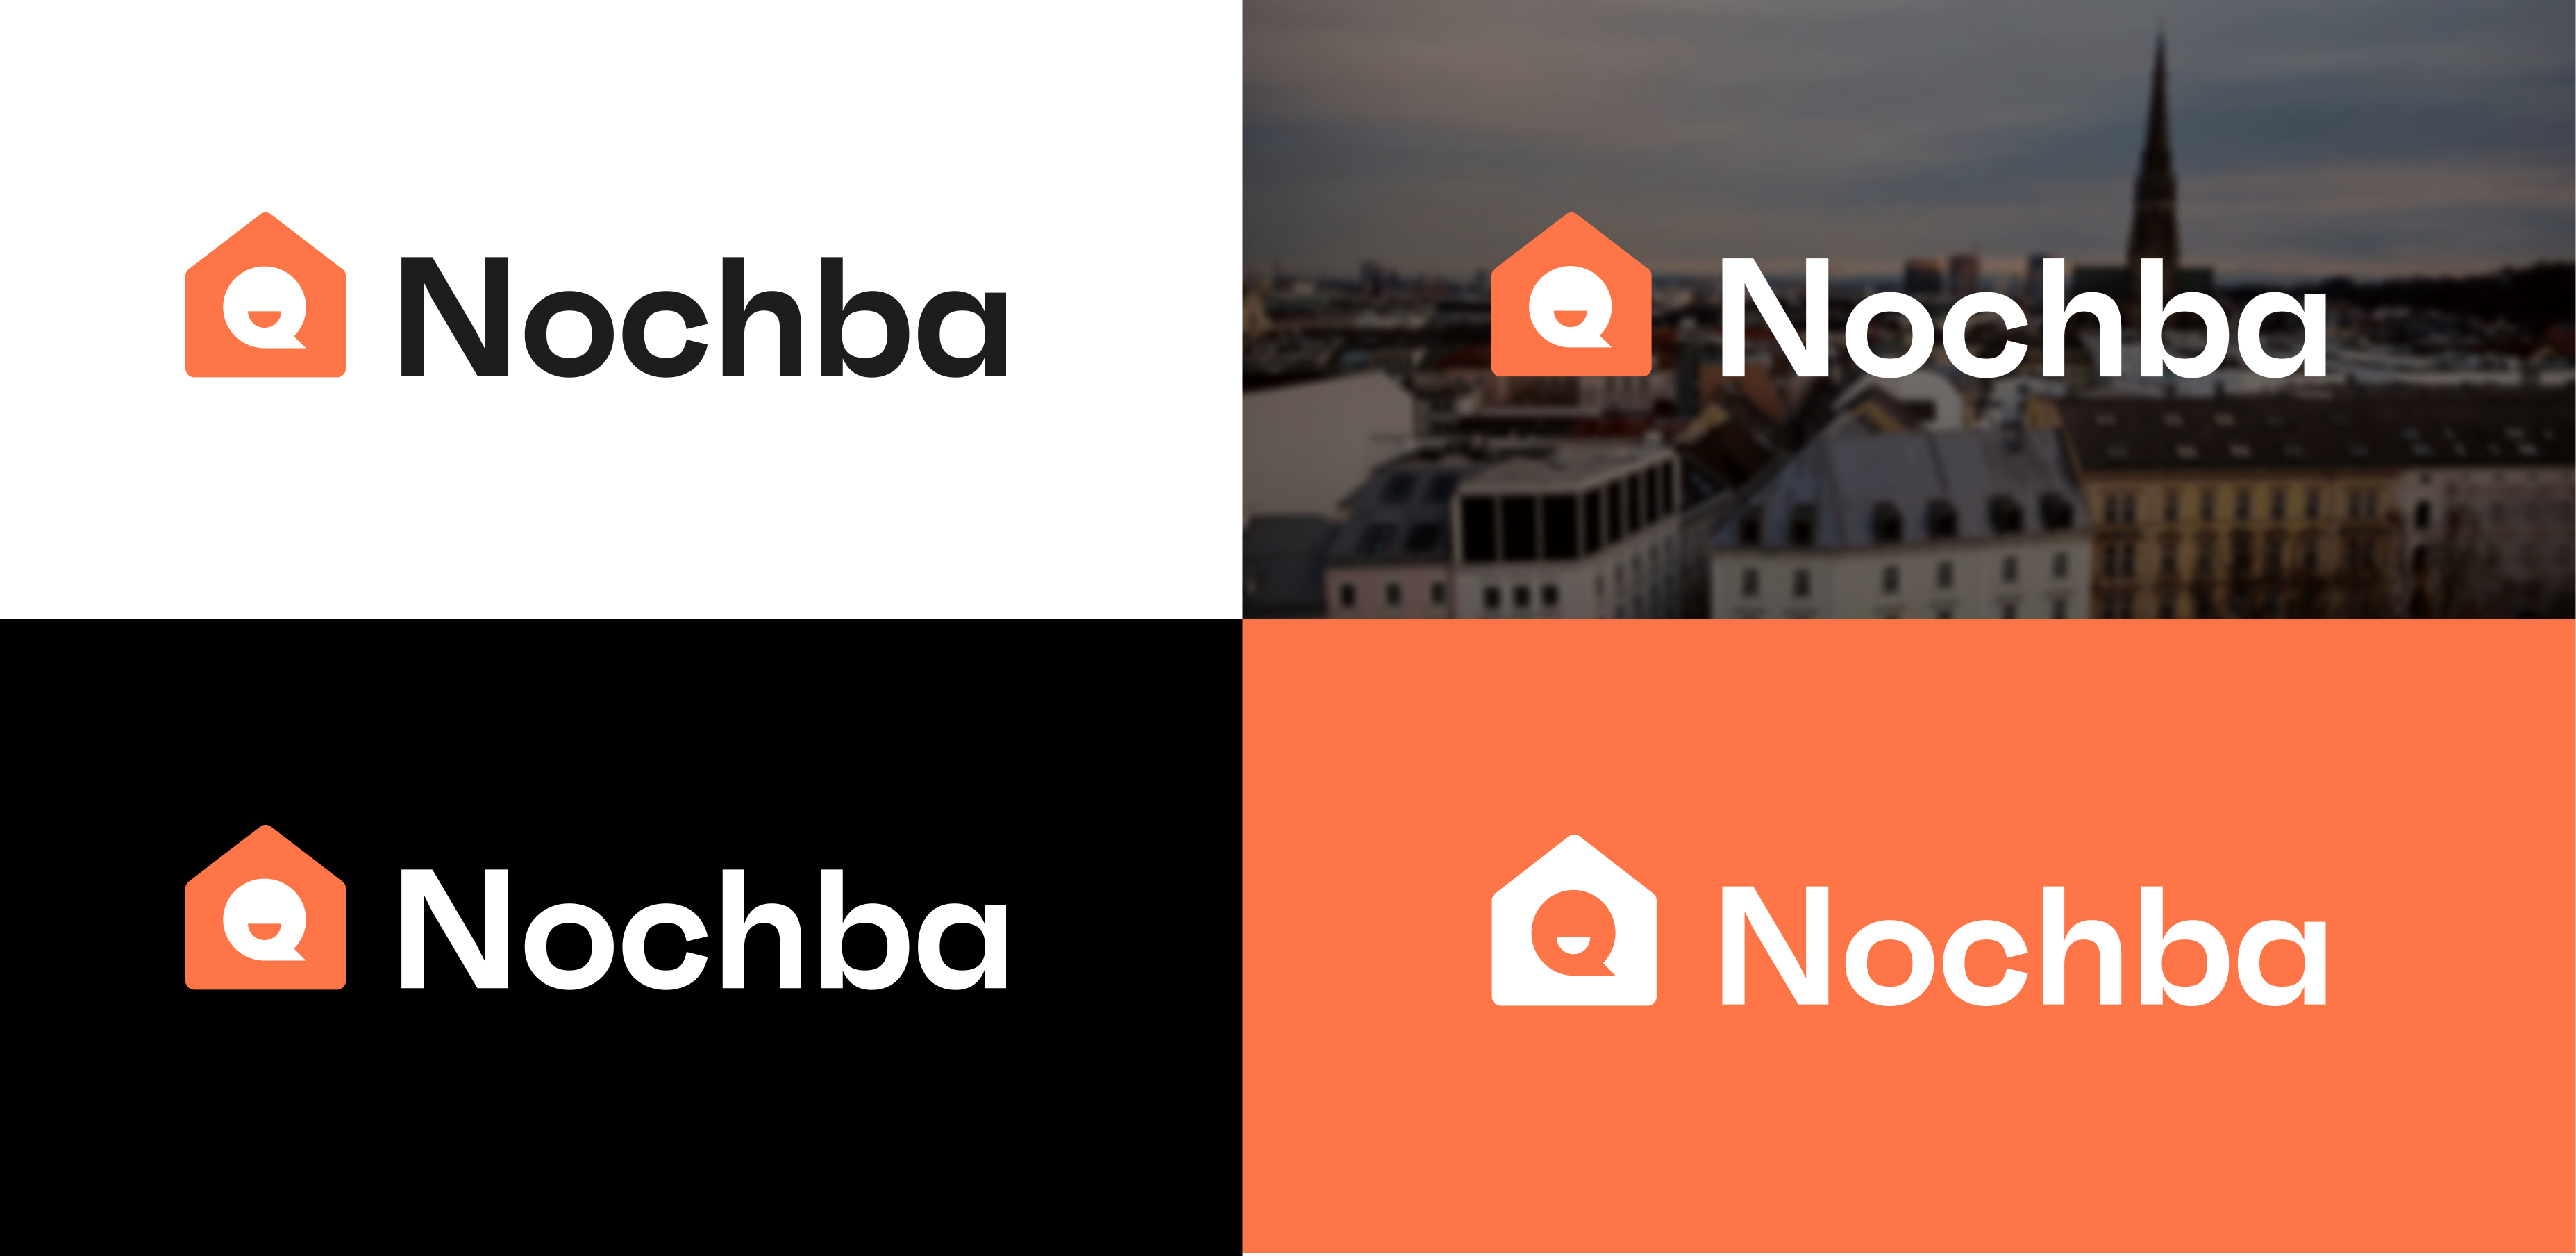
\includegraphics[width=0.95\textwidth]{pics/final-logo.png}

% 
\includegraphics[width=0.35\textwidth]{pics/app-logo.png}

% überschrift logo historie
\paragraph{Logo Historie}



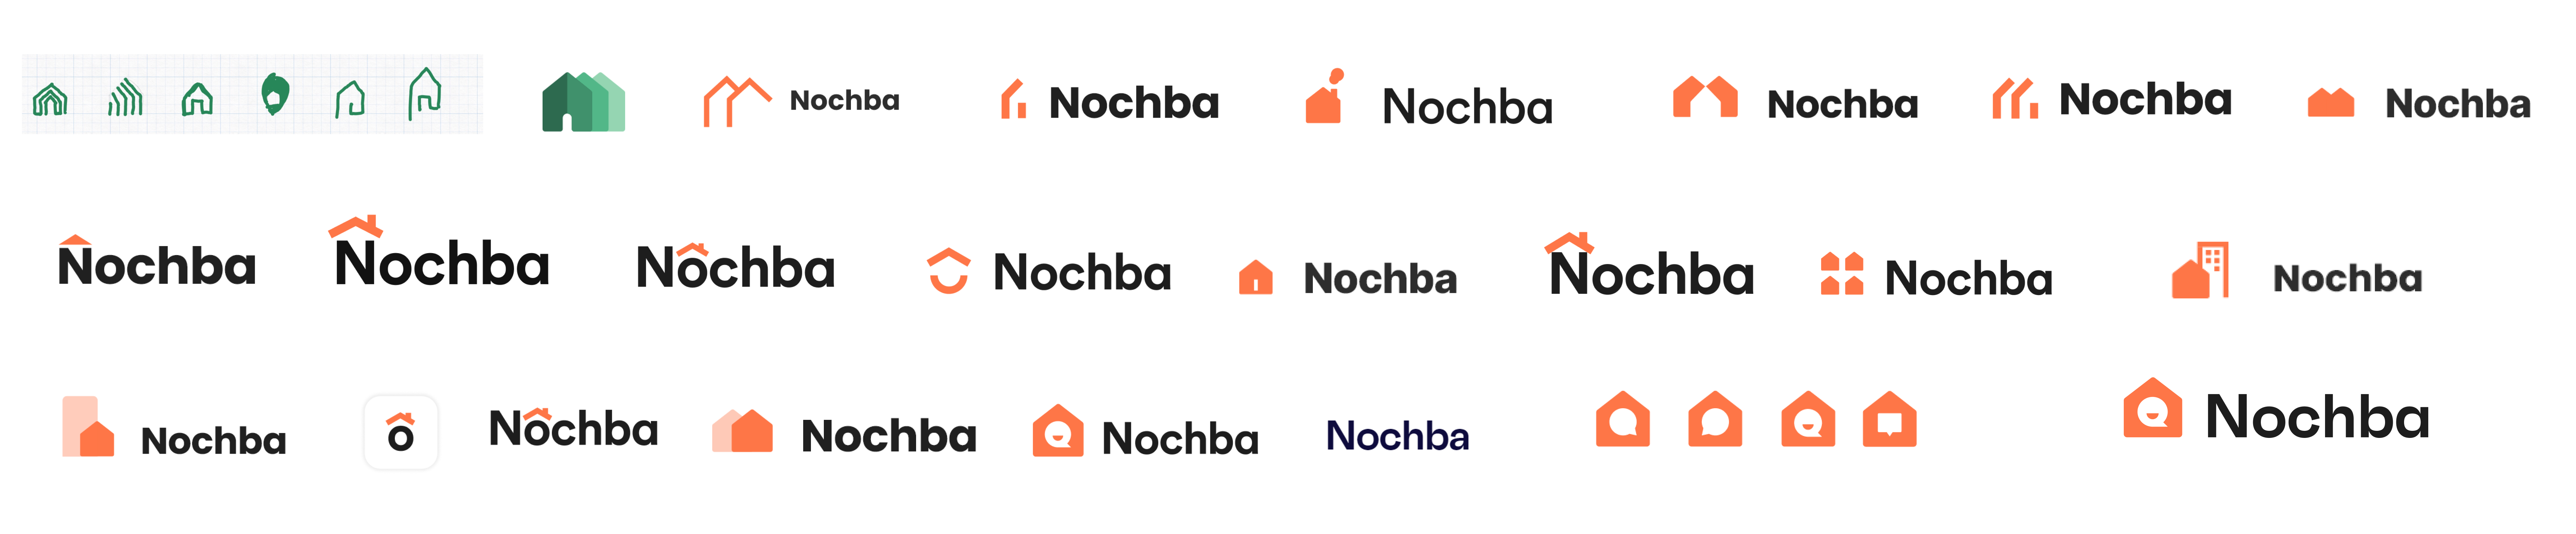
\includegraphics[width=0.95\textwidth]{pics/logo-historie.png}



Im Zuge des Designprozesses haben wir hohe Ansprüche an das
Logo unserer App gestellt, da das logo unser Projekt repräsentiert. Es war uns wichtig, dass es einfach gehalten
und leicht erkennbar ist. Wir haben uns Zeit gelassen, um
den endgültigen Entwurf des Logos zu finalisieren, da uns
die vorherigen Entwürfe nicht vollständig zufrieden
stellten. Ich habe gezielt nach anderen Logos gesucht, die
eine Verbindung zu Nachbarschaften oder Häusern herstellen
und Ideen auf unserem Discord-Server gespeichert. Es sollte
immer ein Haus erkennbar sein, da Häuser schnell mit
Nachbarschaften in Verbindung gebracht werden.

In den früheren Versionen der App hatte ich Schwierigkeiten, ein ansprechendes App-Icon zu gestalten, da ich kein eigenständiges Icon hatte. Aus diesem Grund habe ich mich dazu entschlossen, den Schriftzug und das App-Icon (Logo) separat zu gestalten, wie es auch bei anderen Apps üblich ist. Das endgültige Logo habe ich dann erst Ende 2022 entworfen, da mir alle anderen Designs nicht gefielen. Es ist ein Haus mit einer sprechenden Sprechblase, die lächelt, geworden. Dies soll symbolisieren, dass man innerhalb des Hauses sprechen kann und das Lächeln soll verdeutlichen, dass man Freude mit seinen Nachbarn teilen kann. Generell hat ein Lächeln immer eine positive Wirkung auf den Betrachter und es verdeutlicht, dass es sich bei unserer App um eine Anwendung für den Austausch unter Menschen handelt.

Wir haben bewusst eine runde, verspieltere Schriftart gewählt, da sie besser mit der Farbmischung harmoniert als die vorherige Schriftart.
\subsection{App Design}
\subsubsection{Thumb Zone Prinzip}
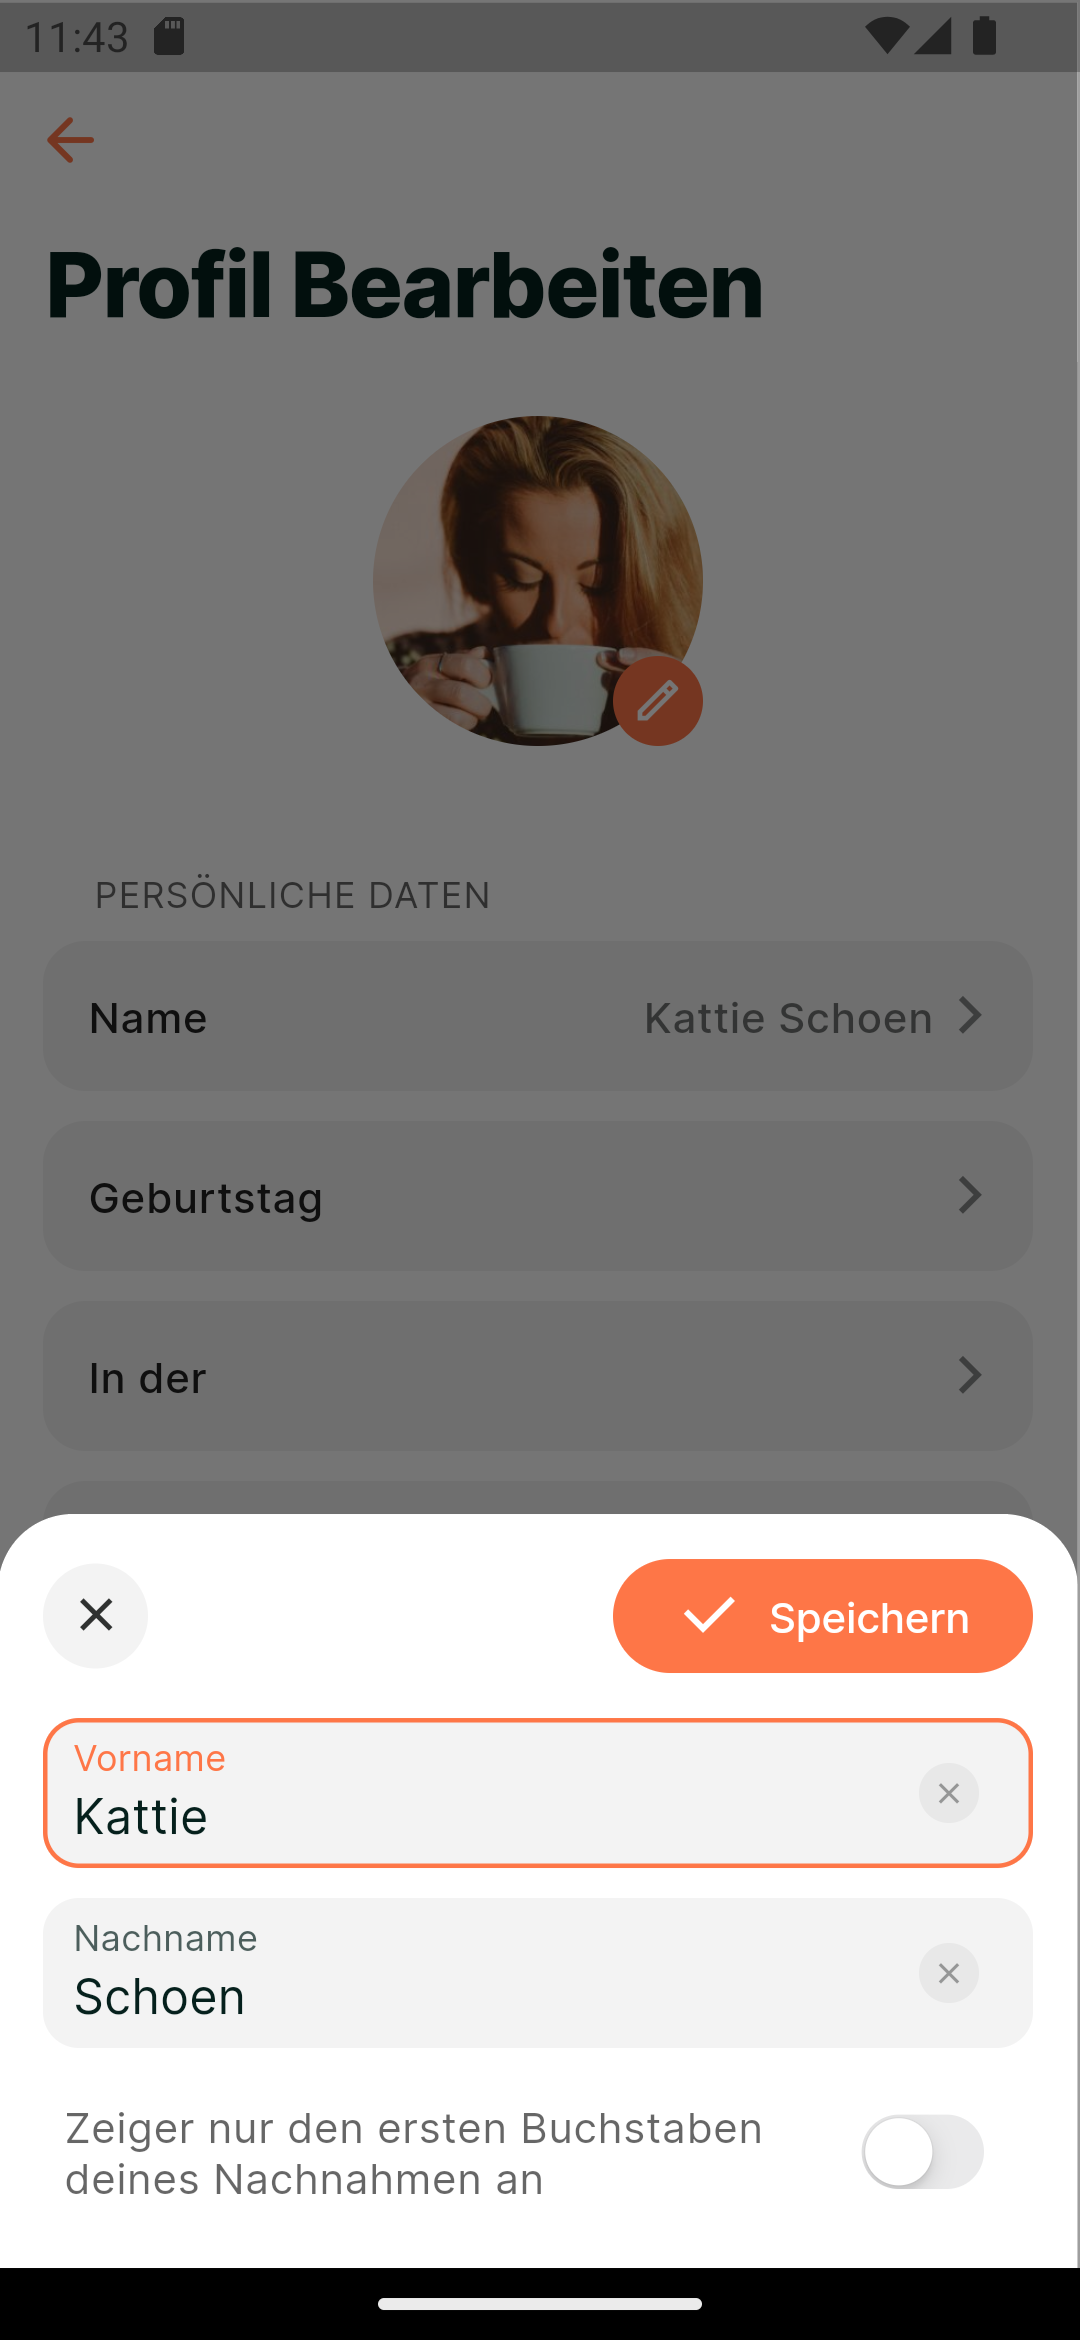
\includegraphics[width=0.3\textwidth]{pics/edit-name-screen.png}
Wir haben versucht, das Thumb Zone Prinzip in unserem Design-Muster zu implementieren, indem wir wichtige UI-Elemente immer im unteren Bereich der App platziert haben. Wenn man die Abbildung betrachtet, kann man deutlich erkennen, dass wir das Layout für die Namensbearbeitung extra unten platziert haben, um alle Klick-Elemente bequem mit dem Daumen bedienen zu können. Wir haben auch alle wichtigen Buttons wie "Speichern" in unserer primären Farbe gestaltet und rechts ausgerichtet, um einen leichteren Zugriff zu gewährleisten. Außerdem haben wir es bei unserer App so implementiert, dass man das Textfeld nicht durch Klicken ändern muss, sondern einfach die Enter-Taste auf der Tastatur drücken kann, um das Eintippen von Daten zu erleichtern. Unwichtige Buttons haben wir in grau gestaltet, wie z.B. den X-Button in der Abbildung. Ein kleines, aber nützliches Feature, das wir eingebaut haben, ist der Löschen-Button neben dem Textfeld, der es dem Benutzer ermöglicht, den gesamten Text bequem zu löschen. Leider ist uns gegen Ende die Zeit ausgegangen, um diese Prinzipien vollständig umzusetzen. In zukünftigen Versionen der App möchten wir sicherstellen, dass diese Prinzipien einheitlich angewendet werden.
\subsubsection{Design Historie}

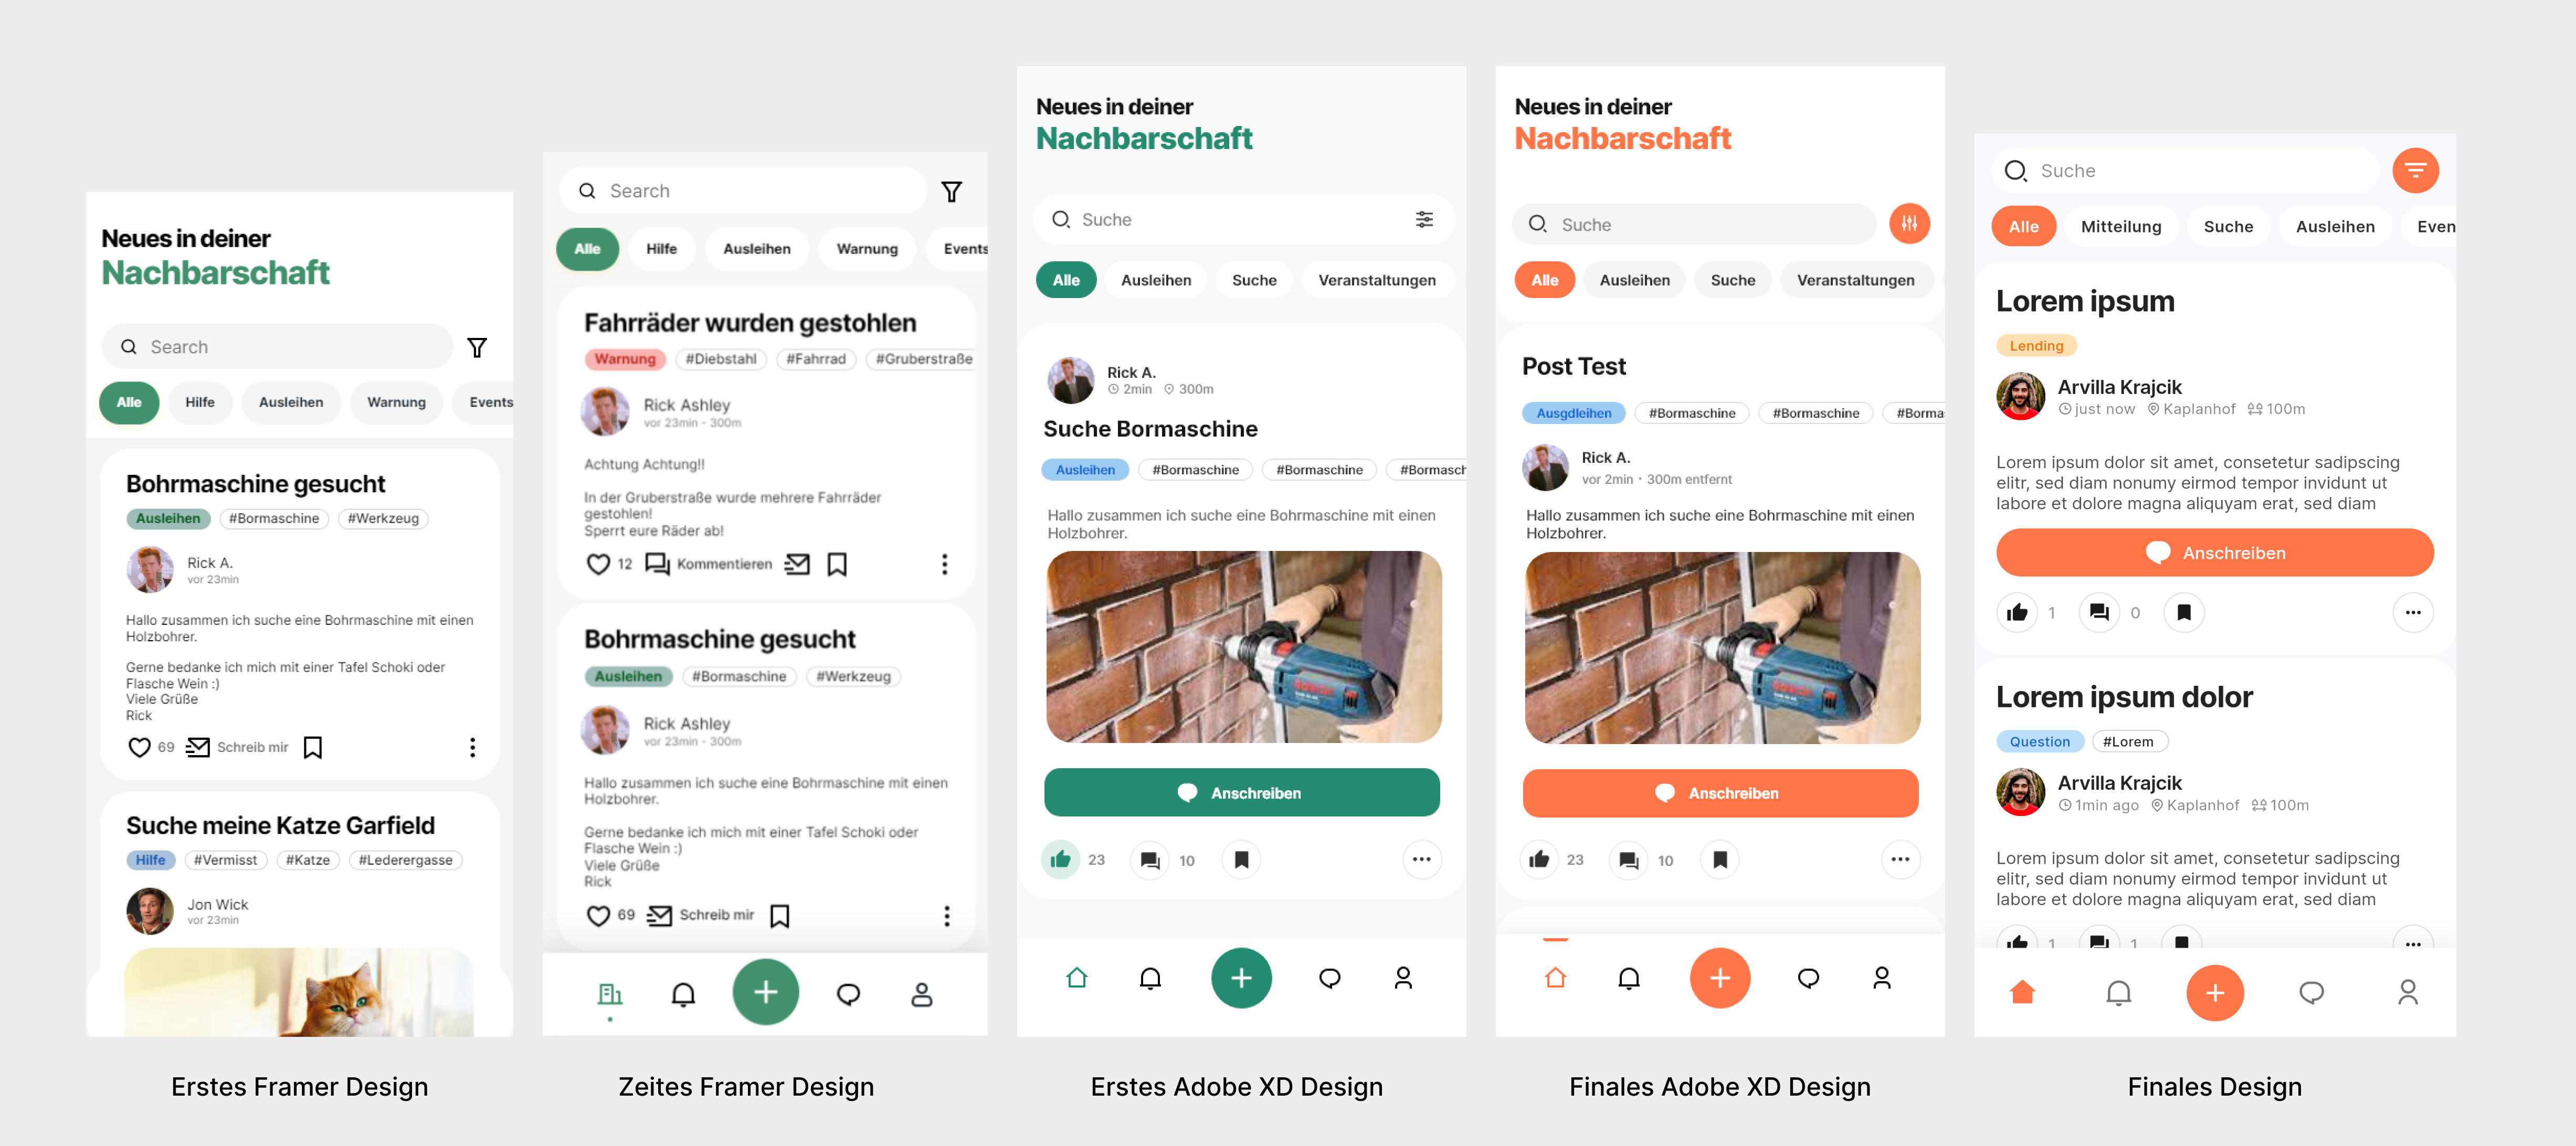
\includegraphics[width=0.95\textwidth]{pics/app-design-history.png}

eingehen mit fotos und beschreibung auf die haupt screens der app

\subsection{Websiten Design}
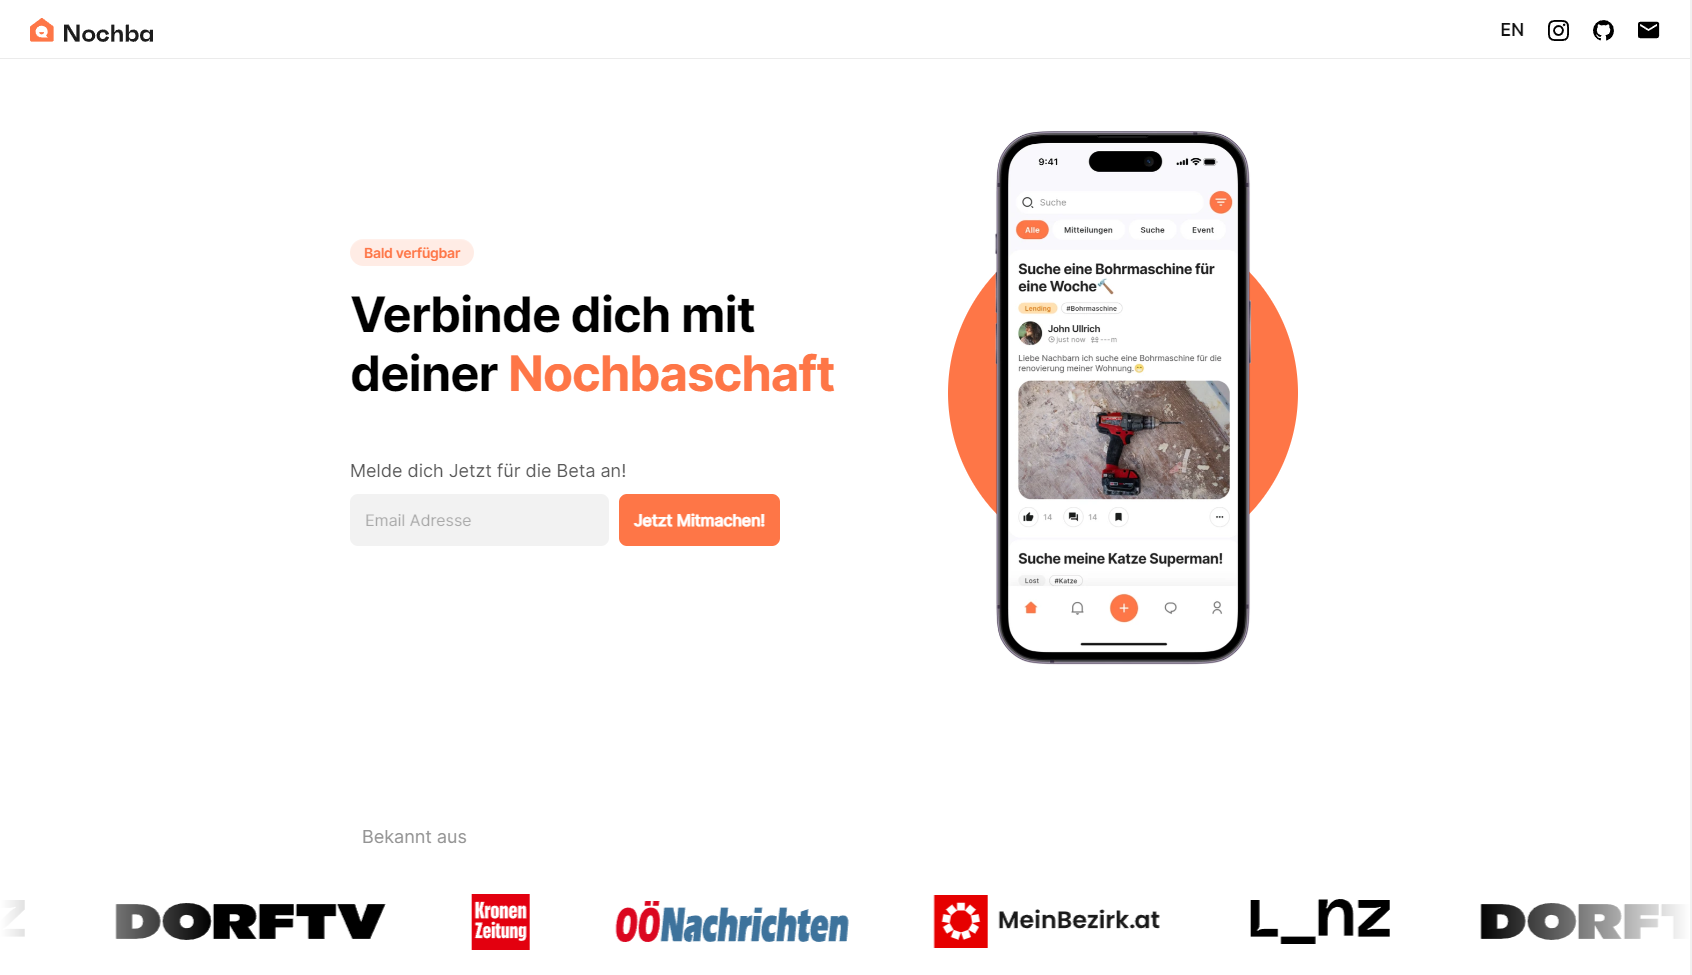
\includegraphics[width=1\textwidth]{pics/website-design.png}


Da unser Projekt aufgrund unserer Teilnahme an Linz hackt in den Medien präsent war und wir keinen zentralen Anlaufpunkt für Informationen hatten, haben wir uns entschlossen, eine schlichte Landing Page mit grundlegenden Informationen zu gestalten. Das wichtigste Feature unserer Website ist die Möglichkeit für Nutzer, sich für die Testphase zu registrieren. Bei der Gestaltung der Landing Page ließ ich mich von den Vorlagen von Framer inspirieren und nutzte hauptsächlich fertige Abschnitte. Wir hielten uns an unsere Farbpalette und achteten darauf, dass die Webseite möglichst einfach gestaltet ist. Ursprünglich hatten wir nicht geplant, eine Website für unser Projekt zu erstellen.

\section{Backend}

\subsection{Firebase}
\author{Martin Hausleitner}
Firebase ist ein BaaS, das uns Entwicklern eine erhebliche Menge an Stress abnimmt. Das Hosting von Datenbanken oder in unserem Fall Cloud-Funktionen funktioniert mit nur wenigen Klicks. Wir müssen uns keine Gedanken über Skalierung oder Ausfälle machen. Unser Firebase-Backend hosten wir auf der Google Cloud in Frankfurt (EUR3 Europe-West), um eine geringe Latenz zu gewährleisten. Zu Beginn haben wir den kostenlosen Plan "Spark" genutzt, was für uns ausreichend war, da wir noch nicht die Firebase-Cloud-Funktionen genutzt haben. Um Geld zu sparen, haben wir dann lange Zeit mit dem lokalen Firebase-Emulator an den Cloud-Funktionen gearbeitet. Im Januar 2023 sind wir dann auf den "Blaze"-Plan umgestiegen, um die Firebase-Cloud-Funktionen nutzen zu können. Bis zum Stand März 2022 haben wir nur wenige Euro für den Verbrauch gezahlt. Wir waren auch sehr beeindruckt von der exzellenten Dokumentation und den vielen Tutorials auf YouTube, die Firebase anbietet.


\subsubsection{Firebase SDKs}
\author{Sandin Habibovic}
Firebase-Tools

\subsubsection{Firebase Authentication}
\author{Sandin Habibovic}
Email und Passwort authentication

\subsubsection{Cloud Firestore}
\author{Sandin Habibovic}
NoSQL-Database, Dokument-basierte Speicherung, Subcollections
\subsubsection{Cloud Storage}
\author{Sandin Habibovic}
Speicherung von Profilbilder und Post-Bilder
\subsubsection{Firebase Cloud Functions}
\author{Martin Hausleitner}
Firebase Cloud Functions sind eine großartige Möglichkeit,
um Business-Logik abzubilden. Es handelt sich um serverlose
Funktionen, die in JavaScript oder TypeScript geschrieben
werden und einzeln auf der Google Cloud gehostet werden. Je
nach Nachfrage werden sie automatisch skaliert oder komplett
abgeschaltet. Ein Nachteil ist, dass die Startup-Zeit länger
sein kann als bei einem herkömmlichen Backend, das immer
läuft. Allerdings kann man durch Cloud Functions viel Geld
sparen, da nur die Prozessorlaufzeit bezahlt werden muss.

Firebase Cloud Functions ermöglichen es Entwicklern, auf verschiedene Ereignisse in Firebase-Produkten zu reagieren. Zum Beispiel, wenn sich Daten in der Firestore-Datenbank ändern oder ein neuer Nutzer in Firebase Authentication registriert wird. Wenn ein solches Ereignis eintritt, wird die entsprechende Cloud Function automatisch ausgeführt.

Wir haben alle Cloud Functions in TypeScript programmiert,
da TypeScript Typsicherheit und erweiterte Fehlererkennung
bietet.


jeder schreibt über seine CF

\subsection{Algolia Search}
\subsection{Algolia SDK}

\subsubsection{Typesense Search}
\subsection{Typesense SDK}
